\documentclass[11pt]{article}
\usepackage[margin=1in]{geometry}
\usepackage[T1]{fontenc}
\usepackage[utf8]{inputenc}
\usepackage{lmodern,microtype,amsmath,amssymb,booktabs,graphicx}
\usepackage[authoryear,round]{natbib}
\usepackage[hidelinks]{hyperref}
\hypersetup{pdftitle={Trial Ledger: Auditing Adaptive Agent Backtests},pdfauthor={Nicolas Coquelet}}
\newcommand{\CorrectedEpisodes}{265}
\newcommand{\CliTotal}{105}
\newcommand{\CliValidNull}{100}
\newcommand{\CliNaive}{86}
\newcommand{\CliLedger}{0}
\newcommand{\NimValidNull}{118}
\newcommand{\NimNaive}{109}
\newcommand{\NimLedger}{1}
\newcommand{\NimUnder}{65}
\newcommand{\NimClaims}{117}
\newcommand{\MaxUnder}{15.640}
\newcommand{\PrimaryDecisionSentence}{Claimed- and ledger-count DSR decisions differ in 0/217 valid paired null picks at the primary threshold.}
\newcommand{\SpeedLow}{182}
\newcommand{\SpeedHigh}{1,136}
\newcommand{\ResearchStart}{2018-01-01}
\newcommand{\ResearchEnd}{2023-12-31}
\newcommand{\TestStart}{2024-01-01}
\newcommand{\TestEnd}{2026-09-30}
\newcommand{\ProtocolCommit}{5dcf789a}
\newcommand{\AnalysisCommit}{b9cf14499d4d}
\newcommand{\VerifiedTests}{138}
\newcommand{\VerifiedRustTests}{3}
\newcommand{\VerifiedCiCommit}{b9cf1449}
\newcommand{\StoredLedgers}{265}
\newcommand{\StoredTrials}{36,163}
\newcommand{\StoredObjects}{29,609}
\newcommand{\RustOriginalMs}{219.863}
\newcommand{\RustFinalMs}{189.664}
\newcommand{\EthSelections}{25}
\newcommand{\EthRules}{15}
\newcommand{\EthEvaluations}{16}
\newcommand{\EthCodexRules}{1}
\newcommand{\EthCodexLater}{1.403}
\newcommand{\EthReferenceLater}{0.423}

\title{Trial Ledger: Auditing Adaptive Agent Backtests}
\author{Nicolas Coquelet\\CentraleSupélec \& ESSEC Business School}
\date{October 2026}

\begin{document}
\maketitle
\begin{abstract}
An agent's final backtest does not reveal how many alternatives preceded it.
We instrument a constrained strategy-search environment with an anchored,
hash-chained trial ledger and compare self-reported counts with distinct
recorded return series. A corrected, fixed-plan study contains
\CorrectedEpisodes{} search attempts, including \CliTotal{} real Codex CLI
sessions using \texttt{gpt-6.1-sol} and three hosted NIM models. On constructed
zero-conditional-mean markets, naive probabilistic Sharpe ratio acceptance is
\CliNaive/\CliValidNull{} for Codex and \NimNaive/\NimValidNull{} for NIM;
ledger-count deflation accepts \CliLedger/\CliValidNull{} and
\NimLedger/\NimValidNull{}, respectively. NIM null-market self-reports under-count trials in
\NimUnder/\NimClaims{} usable claims, with maximum ratio \MaxUnder{}.
\PrimaryDecisionSentence{}
The study does not establish general trading ability or universal statistical
calibration. An independent audit exposed future-dependent sizing in the first
version; we retain that evidence as superseded and rerun adaptive searches with
fixed, causal sizing. The BTC evaluation period had already been examined and
is a post-review diagnostic. A separate Rust CSCV benchmark achieves
\SpeedLow--\SpeedHigh$\times$ speedups over memory-feasible pypbo cases on one
isolated Linux runner, with output checks. Code, cached responses, anchored
ledgers, compressed returns and generated paper inputs accompany the study.
\end{abstract}

\section{Introduction}
Backtesting permits repeated selection against a fixed historical sample.
A search can therefore produce an apparently compelling strategy on a market
with no predictable mean return. Tool-using language models automate this
search, but their final explanations need not account for every parameter-grid
evaluation. A tool invocation is not necessarily a statistical trial: one sweep
can evaluate many configurations, while repeated calls can evaluate identical
returns. Deflation requires an explicit convention for the trial universe.

We study accounting and selection within a small, inspectable environment.
The final candidate is the agent's submitted specification, including cases
where that specification is invalid or absent from its own search ledger.
We compare a single-trial acceptance statistic with the same deflation formula
using either the agent's claimed count or the ledger's distinct-return count.
These are different questions: correcting for search may reject a naive winner,
yet replacing a claimed count with a verified count may change no decision.

The contributions are:
\begin{enumerate}
\item An MCP service, shell-capture path and execution wrapper that record
individual evaluations before feedback, with externally anchored chain heads
and content-addressed return objects.
\item A fixed-plan comparison of hosted tool loops and real CLI sessions,
reporting attempts, failures, count discrepancies, paired decisions and
uncertainty rather than only successful backtests.
\item An allocation-conscious Rust implementation of combinatorially symmetric
cross-validation (CSCV), with separately licensed reference comparisons,
output checks and binary notice audits.
\end{enumerate}
The statistical tests are established methods, not new estimators. The evaluation
is restricted to predefined strategy families, a single data source and specified
agent configurations.

\section{Related work}
\citet{dsr} develop the Deflated Sharpe Ratio (DSR) to account for selection and
non-normal return moments. \citet{pbo} introduce probability of backtest
overfitting (PBO) and CSCV, which assesses the out-of-sample rank of an
in-sample winner across symmetric partitions of a candidate-return matrix.
We implement these constructions and expose the counted trial universe;
we do not interpret either statistic as protection against every source of
leakage or dependence.

\citet{gencay} is the closest related work on search-aware evaluation of
LLM-discovered trading strategies. That work combines restricted tools,
recorded evaluations and statistical deflation, and explicitly distinguishes
leakage prevention from search correction. Our narrower contribution is an
auditable capture interface, a direct comparison of claimed and recorded
counts, and real CLI subjects alongside hosted chat-model tool loops.
The independent audit of our initial sizing rule illustrates why lagging a
signal is insufficient if another component uses future observations.

The Python package \href{https://github.com/esvhd/pypbo/tree/4d723f06498267a2a6280cb9d7d5649348e961d1}{pypbo}
is a software benchmark reference, fetched at a fixed commit under its separate
AGPL licence. Its source is not incorporated into the MIT runtime.
\citet{bootstrap} provide the stationary bootstrap used to construct one null
market. Wilson intervals \citep{wilson}, paired-proportion comparisons
\citep{mcnemar} and signed-rank comparisons \citep{wilcoxon} provide descriptive
uncertainty and paired analyses; their assumptions are stated below.

\section{Data}
We use Binance spot BTCUSDT daily closes. The research window is
\ResearchStart{} through \ResearchEnd{}; the subsequent diagnostic period is
\TestStart{} through \TestEnd{}. The committed download and normalization
script handles the source timestamp formats, and data checksums identify the
exact input file. No Yahoo or Kaggle data enter this experiment.
Binance-derived data and figures retain the dataset's non-commercial/share-alike
restrictions and attribution, separately from the MIT code licence.\footnote{Source terms and attribution:
\url{https://github.com/binance/binance-public-data/blob/master/TERMS_AND_CONDITIONS.md}.
Exact licence receipts and handling are in \texttt{THIRD\_PARTY\_NOTICES.md}.}

Two synthetic markets use only the BTC research period for calibration. The
signflip market samples absolute daily returns using a stationary bootstrap
with mean block length 20 and multiplies them by independent symmetric signs.
The second market follows a zero-mean GARCH(1,1) recursion \citep{garch} with standardized
Student-$t$ innovations and symmetric clipping of returns. Each null has
2,190 scored daily observations. Parameters and generated GARCH inputs are
frozen; retaining only fitted parameters was insufficient for byte-exact
cross-platform reproduction of the Student-$t$ sampler.
\begin{table}[tbp]
\centering\small
\setlength{\tabcolsep}{4pt}
\caption{Frozen zero-mean GARCH calibration using demeaned BTC research returns. The persistence constraint is active to numerical precision.}\label{tab:data}
\begin{tabular}{rrrrr}
\toprule
$\omega$ & $\alpha$ & $\beta$ & $\nu$ & Persistence cap \\
\midrule
6.842864e-06 & 0.0595577 & 0.9354423 & 3.417848 & 0.995 \\
\bottomrule
\end{tabular}
\end{table}

The fitted persistence reaches the imposed cap. This is a descriptive synthetic
control, not a claim that the fitted process adequately models BTC. Clipping is
symmetric, preserving the zero conditional mean.

Independent signs or symmetric innovations imply zero conditional expected
market return before costs. For any fixed strategy with predictable positions,
expected gross strategy return is also zero. Selecting a specification after
seeing the research window can nevertheless produce a positive realized
Sharpe ratio. This post-selection effect is the intended null experiment.

\section{Method}
\subsection{Causal backtests and capture}
The rule families are momentum, moving-average crossover, mean reversion,
breakout and RSI, with long-only and volatility-targeting modifiers. A signal
computed at close $t$ sets the holding for observation $t+1$. Net returns are
\begin{equation}
 r^{\mathrm{strat}}_{t+1}=p_t r_{t+1}-c|p_t-p_{t-1}|,
 \qquad c=5\times10^{-4}.
\end{equation}
Volatility targeting multiplies the base signal by
$\min(2,0.02/\widehat\sigma_{t,20})$, using the trailing 20 observations
available at close $t$. The fixed per-period target is not fitted to either
research or diagnostic data. Positions are zero during unavailable warm-up.
Tests perturb future observations and require equality of full position sizes
and preceding returns, including a diagnostic-period prefix.

Each successful backtest is appended before its feedback is returned. A sweep
records every valid configuration. The ledger stores strategy and engine hashes,
dataset and time-axis identity, sampling frequency, moments, returns hash and
chain links. The episode receipt anchors the terminal sequence and hash outside
the subject workspace. Compressed float64 returns are addressed by the hash of
their canonical uncompressed content. An actor able to rewrite both a ledger
and its only anchor can rebuild a consistent history; this is tamper evidence,
not an adversarial execution sandbox.

Within a coherent evaluation cohort, ledger $N$ counts distinct evaluated return
series. Unproven identity in a scored shell emission does not justify
deduplication: each such evaluation remains distinct. Public aggregation rejects
mixed datasets, time axes, lengths or frequencies. Legacy records without a time
axis require an explicit, labelled alignment assertion. PBO refuses missing
returns and never selects only the most common series length. Integrity or replay
failure aborts statistical publication.

\subsection{Acceptance and paired counts}
Let $\widehat{SR}$ be the mean return divided by its sample standard deviation,
$T$ the observation count, and $\widehat\gamma_3,\widehat\gamma_4$ sample
skewness and raw kurtosis. The implemented probabilistic Sharpe ratio is
\begin{equation}
\widehat{\mathrm{PSR}}(SR^*)=\Phi\!\left(
\frac{(\widehat{SR}-SR^*)\sqrt{T-1}}
{\sqrt{1-\widehat\gamma_3\widehat{SR}+
(\widehat\gamma_4-1)\widehat{SR}^{\,2}/4}}\right).
\end{equation}
The naive statistic uses $SR^*=0$. DSR uses the zero-null-mean expected maximum
\begin{equation}
SR_0(N)=\sqrt{\widehat V_{SR}}\left[
(1-\gamma)\Phi^{-1}(1-1/N)+\gamma\Phi^{-1}(1-1/(Ne))\right],
\end{equation}
where $\gamma$ is Euler's constant and $\widehat V_{SR}$ is the sample
cross-sectional variance of distinct trial Sharpes; $SR_0(1)=0$. We hold this
variance estimate and the selected candidate's moments fixed when comparing
claimed and ledger counts. Acceptance is strictly greater than 0.95.
These are the implemented plug-in statistics, not a guarantee of calibrated
5\% error under adaptive search, correlated trials or serially dependent returns.

Claimed $N$ is a positive integer in the final answer. Under-reporting means
claimed $N$ is smaller than distinct-return ledger $N$. All positive claims enter
count accounting, including claims accompanying invalid final strategies.
Acceptance denominators include valid completed picks; all planned attempts and
statuses are also reported. No best logged candidate replaces a failed submission.

\subsection{Conditional PBO and implementation}
CSCV splits the research-return matrix into 16 contiguous blocks and considers
all equal-size block selections and their complements. As in the reference
implementation, only the first $16\lfloor T/16\rfloor$ rows enter CSCV; any
short trailing remainder is discarded consistently. For each split it selects
the highest training Sharpe, then computes that column's test rank, with average
ranks for ties. If $w$ is rank divided by $N+1$, the split logit is
$\log(w/(1-w))$, and PBO is the fraction of non-positive logits.
This conditions on the already discovered candidate universe. Agent search is
not repeated inside each fold; PBO does not validate the complete adaptive
selection procedure on fresh data.

The Rust kernel stores block sufficient statistics contiguously, reuses scratch
buffers per rayon chunk, and combines test scoring with rank reduction. It avoids
reconstructing train/test matrices for every split. No fast-math is used. Rust
variants and thread counts are checked for byte-identical output arrays;
comparisons with NumPy and pypbo use recorded exact-PBO and logit-tolerance checks.
The exported purged-fold utility separately removes every training-label interval
intersecting a test-label interval and applies embargo after the union's right
boundary. It is tested but not used to generate the headline experiment.

\section{Protocol}
\subsection{Splits, registration status and correction history}
There is no fitted predictive model or separately tuned validation split.
Agents adaptively choose rule parameters using the research window; search
multiplicity is the object of study. Evaluation code withholds subsequent BTC
rows from the tools. A fixed submitted candidate receives one diagnostic-period
evaluation; offline reproduction repeats its arithmetic.

The first implementation estimated its volatility target from the full supplied
window. Independent review showed that future observations changed preceding
positions and that appending BTC test data changed research-period returns.
Consequently the original study is superseded, including searches whose final
pick did not use that modifier but whose feedback could have been affected.
We retain its receipts and metrics at the original result path. Corrected results
come from fresh adaptive searches, not a retrospective rescore of old winners.

The corrected plan was committed before corrected inference, at
\texttt{\ProtocolCommit}. It is an internal versioned plan, not an externally
registered preregistration. Earlier study outcomes and the BTC period had already
been inspected. We therefore make no untouched-test or independent-confirmation
claim for the corrected BTC results. We disclose both evaluation versions, retain
every logged trial and choose no favourable version, seed or threshold for reporting.
Implementation revisions address demonstrated correctness defects, not
outcome-guided strategy tuning.

\subsection{Subjects and fixed budgets}
The fixed plan contains 100 Codex null attempts (50 seeds on each market) and
five BTC sessions, each in a fresh workspace with isolated MCP configuration.
Codex uses \texttt{gpt-6.1-sol} with medium reasoning. The hosted subjects are
\texttt{openai/gpt-oss-20b},
\texttt{nvidia/nemotron-3.5-lightning-30b-a3b}, and
\texttt{nvidia/nemotron-3-ultra-550b-a55b}, each with 20 seeds per null and five
BTC episodes at temperature 0.7. Random controls have ten seeds per null and
five BTC episodes. Claude Code Haiku is an authentication pilot, reported
separately if inference cannot start.

Each episode has at most 30 backtest tool calls; a sweep may evaluate up to
50 combinations. The running ledger counter is hidden, while sweep sizes remain
visible. CLI subjects may write scratch code but evaluate strategies only through
MCP. The shell hook has a live capture smoke check; scored evaluations here use
MCP. These sessions do not measure unrestricted program synthesis or deliberate
evasion. Provider weight revisions were not pinned; aliases and available CLI
versions are recorded. Market seeds and request-cache salts are not
provider-side inference seeds.

\subsection{Uncertainty and multiplicity}
We report nominal Wilson 95\% intervals for proportions. Because models reuse
market seeds, pooled independent-episode inference is not claimed. A market/seed
cluster bootstrap uses 5,000 replicates and seed 20261029. With zero successes,
its percentile interval can collapse; the Wilson upper bound remains visible.
The precision target concerns cohort-level descriptive Wilson intervals.

Within each model, exact two-sided McNemar tests compare claimed- and ledger-count
acceptance; signed-rank tests compare their continuous DSR scores. Model-specific
continuous-score $p$-values receive Holm step-down correction. For ordered values
$p_{(1)}\le\cdots\le p_{(m)}$, the adjusted value is
$\min\{1,\max_{j\le i}(m-j+1)p_{(j)}\}$. Paired inference assumes independent
market draws; signed-rank interpretation additionally assumes symmetric paired
differences. Zero discordance does not demonstrate equivalence.

Other thresholds, observed score-boundary intervals and hypothetical claimed-count
fractions are exploratory sensitivity analyses. They do not alter the primary
threshold or become observed agent claims. Ledger $N$ captures within-search
multiplicity; it does not by itself account for every upstream model-development
choice or calibrate all dependence assumptions.

\section{Results}
\subsection{Null acceptance and count accounting}
\begin{table}[tbp]
\centering\small
\setlength{\tabcolsep}{4pt}
\caption{Corrected null-market acceptance. Brackets are nominal Wilson 95\% intervals in percent; fractions use valid picks.}\label{tab:cohorts}
\begin{tabular}{lrrrr}
\toprule
Cohort & Attempts & Naive PSR & DSR claimed $N$ & DSR ledger $N$ \\
\midrule
Codex & 100 & 86/100 [77.9, 91.5] & 0/100 [0.0, 3.7] & 0/100 [0.0, 3.7] \\
NIM & 120 & 109/118 [86.1, 95.9] & 1/117 [0.2, 4.7] & 1/118 [0.1, 4.6] \\
\bottomrule
\end{tabular}
\end{table}

\begin{table}[tbp]
\centering\small
\setlength{\tabcolsep}{4pt}
\caption{Null attempts, valid submissions and count accounting. Medians are across attempts or available positive claims; invalid picks retain their claims.}\label{tab:models}
\begin{tabular}{lrrrrr}
\toprule
Subject & Attempts & Valid & Median $N_L$ & Median $N_C$ & Under-reports \\
\midrule
Codex (gpt-6.1-sol) & 100 & 100 & 30 & 30 & 0/100 \\
gpt-oss-20b & 40 & 38 & 170.5 & 109 & 24/37 \\
Nemotron Lightning & 40 & 40 & 185 & 137 & 26/40 \\
Nemotron Ultra & 40 & 40 & 326 & 292 & 15/40 \\
Random control & 20 & 20 & 133 & 174.5 & 0/20 \\
\bottomrule
\end{tabular}
\end{table}

\begin{figure}[tbp]
\centering
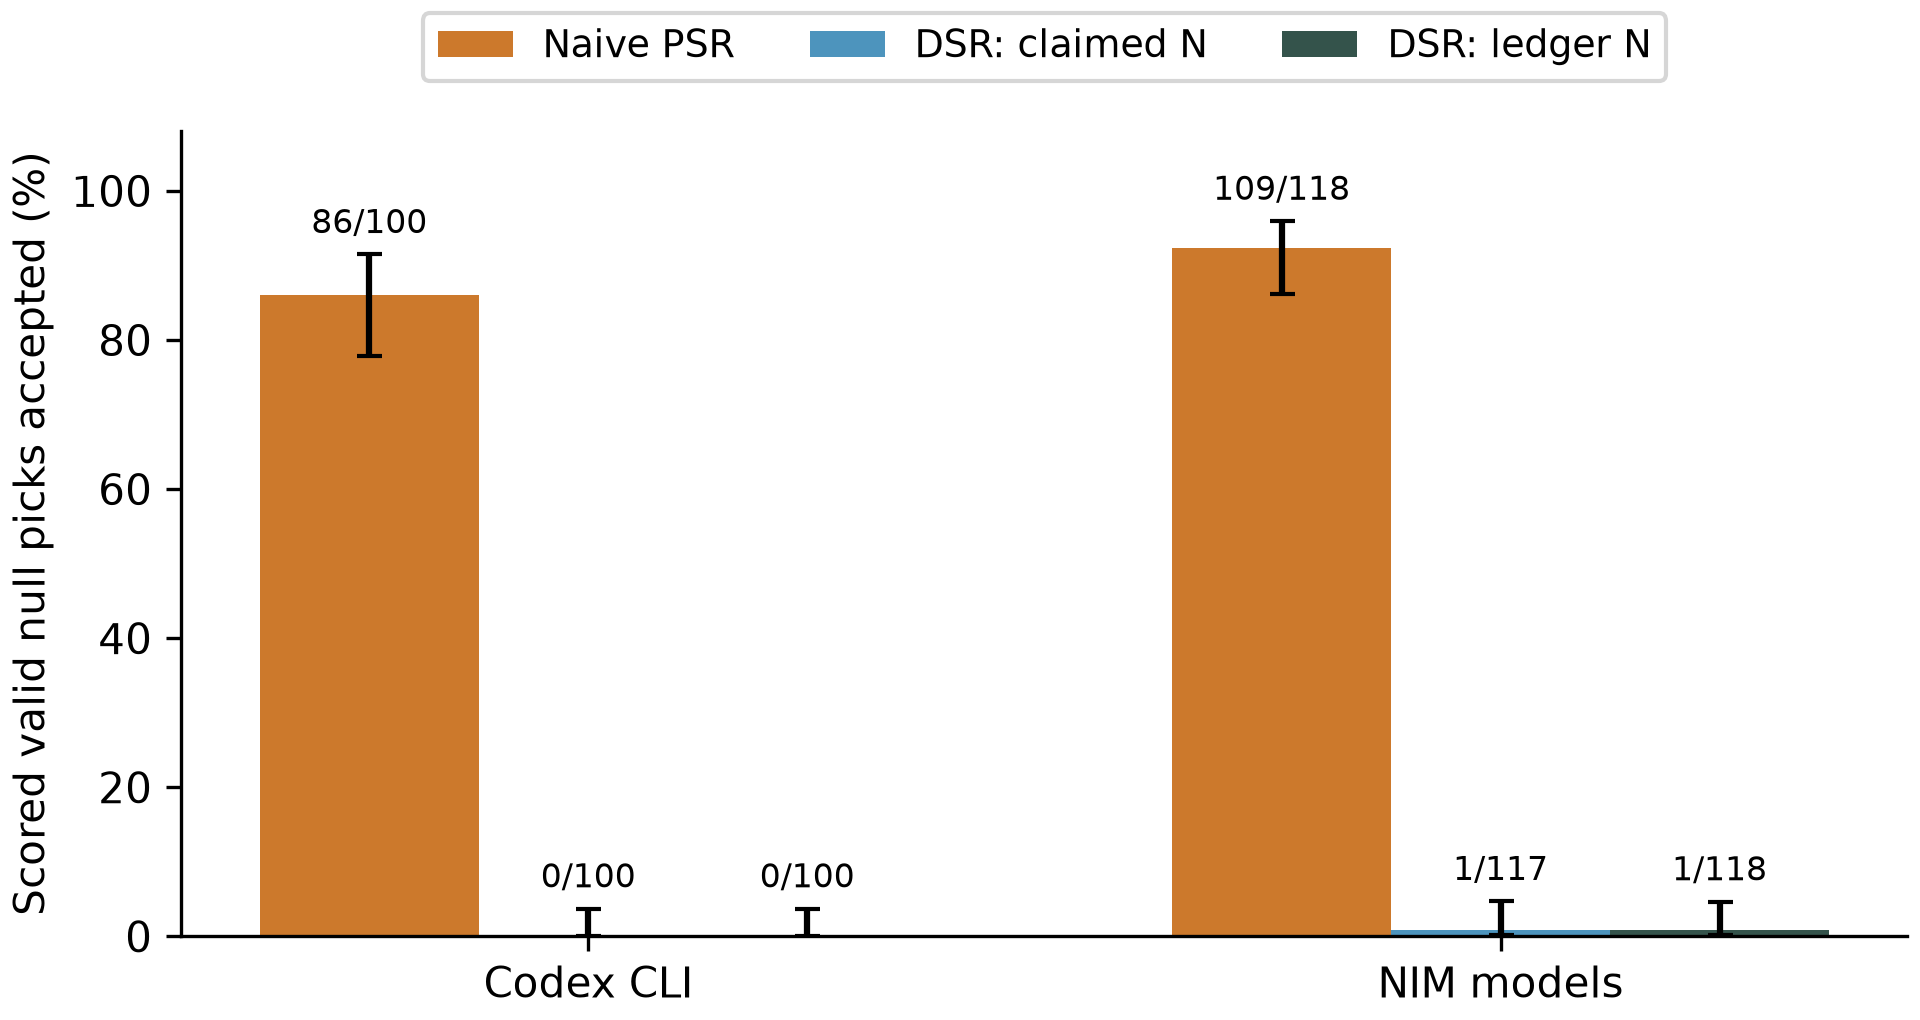
\includegraphics[width=\linewidth]{generated/acceptance.png}
\caption{Corrected null-market acceptance, generated from committed episode and
paired-test results. Bars use valid-pick denominators and nominal Wilson 95\%
intervals. Shared market inputs limit independent-episode interpretation.}
\label{fig:acceptance}
\end{figure}
The acceptance comparison addresses search correction; the claimed-count versus
ledger-count comparison addresses the incremental effect of audited accounting.
\PrimaryDecisionSentence{}
Table~\ref{tab:paired} reports both decision discordance and continuous-score
comparisons. Count errors can change a score without changing a fixed-threshold
verdict. Exploratory counterfactual counts identify possible boundary crossings;
they do not show that an agent actually made the corresponding claim.
\begin{table}[tbp]
\centering\small
\setlength{\tabcolsep}{4pt}
\caption{Primary paired comparisons at 0.95. Discordant decisions and exact McNemar $p$ (unadjusted) are distinct from continuous-score signed-rank tests (Holm adjusted). Parentheses count nonzero score differences used by the signed-rank test. $\Delta=\mathrm{DSR}(N_C)-\mathrm{DSR}(N_L)$.}\label{tab:paired}
\begin{tabular}{lrrrrrr}
\toprule
Subject & \shortstack{Pairs\\(nonzero)} & Claim only & Ledger only & Median $\Delta$ & $p_{McN}$ & $p_{W,Holm}$ \\
\midrule
Codex (gpt-6.1-sol) & 100 (9) & 0 & 0 & 0 & 1 & 0.0154 \\
Nemotron Ultra & 40 (39) & 0 & 0 & -0.00723 & 1 & 0.989 \\
Nemotron Lightning & 40 (40) & 0 & 0 & 0.02623 & 1 & 0.00625 \\
gpt-oss-20b & 37 (36) & 0 & 0 & 0.02357 & 1 & 0.00367 \\
Random control & 20 (20) & 0 & 0 & -0.02473 & 1 & 0.000443 \\
\bottomrule
\end{tabular}
\end{table}

\begin{table}[tbp]
\centering\small
\setlength{\tabcolsep}{4pt}
\caption{Exploratory conditions for differing decisions. Counterfactual counts are floored at one and evaluated at 0.95; they are not observed agent claims.}\label{tab:sensitivity}
\begin{tabular}{lrrr}
\toprule
Scenario & Picks & Claim only & Ledger only \\
\midrule
Observed claims, threshold 0.5 & 217 & 15 & 1 \\
Observed claims, threshold 0.8 & 217 & 1 & 0 \\
Observed claims, threshold 0.9 & 217 & 0 & 0 \\
Observed claims, threshold 0.95 & 217 & 0 & 0 \\
Observed claims, threshold 0.975 & 217 & 0 & 0 \\
Observed claims, threshold 0.99 & 217 & 0 & 0 \\
Hypothetical $N_C=\lfloor 0.5N_L\rfloor$ & 218 & 1 & 0 \\
Hypothetical $N_C=\lfloor 0.25N_L\rfloor$ & 218 & 9 & 0 \\
Hypothetical $N_C=\lfloor 0.1N_L\rfloor$ & 218 & 28 & 0 \\
Hypothetical $N_C=\lfloor 0.02N_L\rfloor$ & 218 & 130 & 0 \\
\bottomrule
\end{tabular}
\end{table}

Across all markets, 3 valid submitted specifications were absent from their episode's recorded search. They are flagged and scored as submitted; no best recorded trial replaces them.
Of 220 planned agent null attempts, 3 lack a usable positive count claim; 1 of these have status ok. Missing or nonpositive counts remain in attempt accounting and are not classified as accurate self-reports.

\begin{table}[tbp]
\centering\small
\setlength{\tabcolsep}{4pt}
\caption{Every attempt status, including the separate authentication pilot.}\label{tab:failures}
\begin{tabular}{llr}
\toprule
Subject & Status & Attempts \\
\midrule
Codex (gpt-6.1-sol) & ok & 105 \\
gpt-oss-20b & api\_error: RuntimeError & 2 \\
gpt-oss-20b & ok & 43 \\
Nemotron Lightning & ok & 45 \\
Nemotron Ultra & ok & 45 \\
Random control & ok & 25 \\
Claude Code Haiku pilot & auth\_failed & 1 \\
\bottomrule
\end{tabular}
\end{table}


\subsection{Previously exposed BTC diagnostic}
\begin{table}[tbp]
\centering\small
\setlength{\tabcolsep}{4pt}
\caption{BTC diagnostic on a previously exposed period. Annualized Sharpe medians use valid submitted rules; repeated rules are counted explicitly.}\label{tab:btc}
\begin{tabular}{lrrrrr}
\toprule
Subject & Attempts & Valid & Rules & Research & Diagnostic \\
\midrule
Codex (gpt-6.1-sol) & 5 & 5 & 1 & 1.167 & 0.552 \\
gpt-oss-20b & 5 & 5 & 4 & 1.236 & 0.616 \\
Nemotron Lightning & 5 & 5 & 4 & 1.167 & 0.552 \\
Nemotron Ultra & 5 & 5 & 3 & 1.388 & 0.796 \\
Random control & 5 & 5 & 5 & 1.299 & 0.629 \\
\bottomrule
\end{tabular}
\end{table}

The test period was examined before the correction. These fixed-specification
results are diagnostic and do not certify trading skill. Multiple sessions can
submit the same rule; the number of distinct specifications is therefore reported
alongside attempts. Differences across versions combine changed sizing and new
adaptive search paths; they are not a paired causal estimate of a correction's
effect on agent ability.

\subsection{Storage and native performance}
\StoredLedgers{} corrected ledgers contain \StoredTrials{} distinct per-ledger
trial series, backed by \StoredObjects{} shared compressed objects. Stored returns
and externally anchored heads verify before analysis. Superseded objects remain
separate from this corrected accounting.
\begin{table}[tbp]
\centering\small
\setlength{\tabcolsep}{4pt}
\caption{Isolated Linux median wall times (ms), two CPU threads. All saved samples contribute; the largest pypbo allocation is skipped.}\label{tab:benchmark}
\begin{tabular}{rrrrrr}
\toprule
$T$ & $N$ & $S$ & Rust & pypbo & Ratio \\
\midrule
1000 & 50 & 8 & 0.119 & 44.149 & 371.0 \\
1000 & 10 & 16 & 3.416 & 3878.965 & 1135.5 \\
2190 & 100 & 10 & 0.588 & 238.172 & 405.2 \\
2190 & 500 & 8 & 1.341 & 244.291 & 182.2 \\
2190 & 1000 & 16 & 189.389 & memory cap & -- \\
\bottomrule
\end{tabular}
\end{table}

The Linux benchmark is a separate fixed-input experiment: two CPU threads,
explicit thread caps, all timing samples retained and a prespecified memory cap.
It runs on a GitHub Actions virtual machine; physical-host contention is not
controlled.
The largest pypbo case is skipped because its estimated allocation exceeds that
cap. The interleaved native comparison improves the largest case from
\RustOriginalMs{} to \RustFinalMs{} ms, with all output arrays byte-identical.
The historical M1 best-run range and the Linux median range use different
hardware and protocols; they are not an improvement comparison. Shared-M1
regressions and unstable timings are retained in the repository. Much of the
advantage over pypbo is algorithmic: the NumPy block-statistics reference also
avoids rebuilding split matrices.

\section{Limitations}
The study uses one prompt, five constrained rule families, a single crypto data
source and a small set of model aliases. It does not establish performance for
arbitrary coding tasks, unrestricted trading programs, other markets or
adversarial agents. Hosted revisions are unknown, and pretrained knowledge of
public BTC history is not excluded by withholding tool access.

The counts are operational definitions, not known independent statistical trials.
Distinct return vectors can remain strongly correlated; identical vectors can
arise from different conceptual hypotheses. The effective-count heuristic is
exploratory. Cross-sectional Sharpe variance estimated from adaptively selected
trials can be too small, and the implemented Sharpe standard error has no HAC
correction. Episode clustering does not correct return-level serial dependence.
Nominal intervals and a negative paired test cannot establish equivalence or a
universal false-discovery guarantee.

PBO conditions on a universe discovered using the full research window. Costs
are a simple fixed turnover charge; fills, funding, liquidation, market impact and operational
risk are not modeled. BTC provides one previously exposed diagnostic period,
with repeated specifications. The correction cannot retroactively recover an
untouched test. Future independent data and a prospectively registered procedure
would be needed for confirmatory generalization claims.

Hash chains require external anchors and trusted capture. The restricted subject
workspaces and prompts do not prove security against malicious escape or trials
performed elsewhere. Shell capture records emitted or recognizable attempts,
not all possible computations. Integrity checks establish consistency with
recorded evidence, not honesty of an arbitrary upstream data provider.

\section{Reproducibility}
The corrected protocol commit is \texttt{\ProtocolCommit}; the analysis source
checkpoint is \texttt{\AnalysisCommit}. Artifact hashes and exact generation
commands are in the committed provenance manifests. Table and figure inputs are
loaded by \texttt{paper/make\_tables.py}, which records their checksums and reads
only committed result blobs. No table cell or empirical headline is hand-entered.
\begin{table}[tbp]
\centering\small
\setlength{\tabcolsep}{4pt}
\caption{Committed source artifacts used by the paper generator. The complete SHA-256 map is in generated/manifest.json.}\label{tab:provenance}
\begin{tabular}{ll}
\toprule
Artifact & Source commit \\
\midrule
Corrected protocol & \texttt{5dcf789a} \\
Episode analysis and stored returns & \texttt{b9cf14499d4d} \\
Linux native benchmark & \texttt{1313f520e666} \\
Review regressions and binary notices & \texttt{b9cf14499d4d} \\
\bottomrule
\end{tabular}
\end{table}

The review-regression checkpoint \texttt{\VerifiedCiCommit} passes
\VerifiedTests{} Python tests and \VerifiedRustTests{} native Rust tests on both
CI platforms, including full-notice checks for both wheels and the source archive.

From the repository root:
\begin{verbatim}
uv sync --all-extras --group dev --group experiments --group bench
uv run --no-sync python -m experiments.run reproduce
uv run --no-sync pytest
CARGO_BUILD_JOBS=2 cargo test --release --manifest-path rust/Cargo.toml
uv run --no-sync python paper/make_tables.py
tectonic -X compile paper/main.tex
\end{verbatim}
Reproduction makes no inference calls: it replays cached NIM responses, regenerates
random controls, audits CLI ledgers and reruns recorded specifications against
return hashes. It does not replay CLI inference. Superseded ledgers receive
integrity checks; their old scores are not recomputed with the corrected engine.
New NIM batches use the shared atomic two-slot limit, one serial requester per
slot, response caching and transient-error backoff. Long-job diagnostics are
ignored locally; research receipts are committed. Both platform wheels and the
source archive contain complete locked native dependency notices, verified before
CI artifact upload. No PyPI publication is performed.

All scientific references have verified DOI or arXiv identifiers in the
bibliography and saved primary-source metadata in
\texttt{paper/reference\_verification.json}. Code is MIT; derived Binance data
and figures retain their separately stated non-commercial/share-alike terms.

\section{Conclusion}
Trial accounting makes adaptive backtest search inspectable. The experiment
separates naive acceptance, search deflation and the incremental effect of
replacing a self-report with a recorded count. \PrimaryDecisionSentence{}
A verified count is useful evidence even when it changes no threshold decision.
The correction history also shows that statistical deflation cannot substitute
for causal evaluation code. The accompanying ledgers, return objects and
reproduction checks support auditing the reported calculations within their
stated scope; they do not establish a profitable trading system.

\bibliographystyle{plainnat}
\bibliography{refs}
\end{document}
